\documentclass[main.tex]{subfiles}
\begin{document}
\subsection{Day 21: 10/12/22}
Let's talk about the motivation from single-variale calculus:

\begin{definition}[Single-variable limits of functions]
    Consider $a_0 < a < a_1$, $A = (a_0, a) \cup (a, a_1)$ or $A = (a_0, a_1)$, and $f : A \to \RR$. Then we define \vocab{$\lim_{x\to a} f(x) = y$} if and only if for all $\varepsilon > 0$ there exists $\delta > 0$ such that $\abs{f(x) - y} < \varepsilon$ for all $x\in A$ with $0 < \abs{x - a} < \delta$.
\end{definition}

Before we move on to limits in $\RR^n$, let's introduce the notion of accumulation points so that the limit point cannot just be anywhere in our domain; note that we can essentially disregard this with open sets.

\begin{definition}
    Let $A\subseteq \RR^n$, $\vec{a}\in \RR^n$. We say that $\vec{a}$ is an \vocab{accumulation point} of $A$ if $A\cap B_\rho\parens{\vec{a}}\setminus \braces{\vec{a}} \neq \emptyset$ for all $\rho > 0$.
\end{definition}

Basically, the blue shaded area must be nonzero for any $\rho > 0$ in the following image for $\vec{a}$ to be an accumulation point:

\begin{center}
    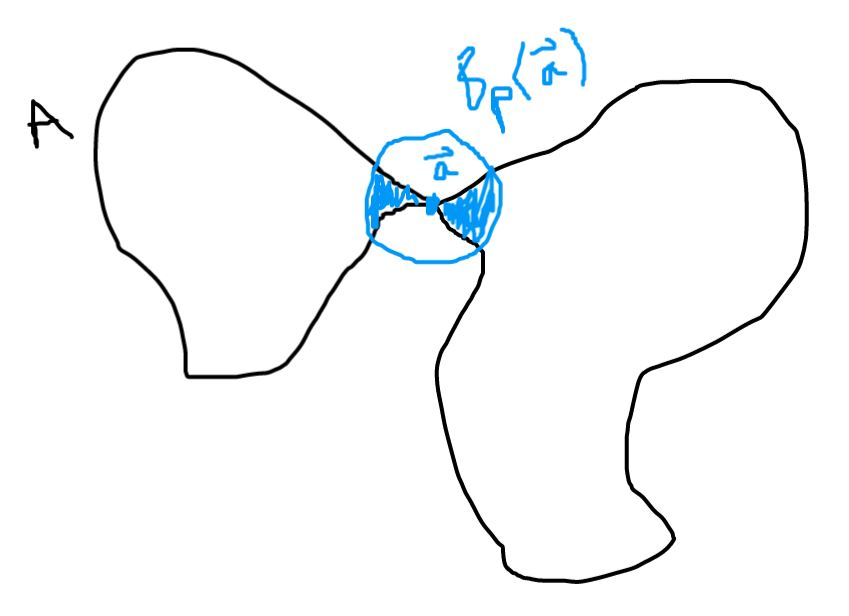
\includegraphics[width = 0.7\textwidth]{accumulation_point.JPG}    
\end{center}

Basic properties of accumulation points:
\begin{enumerate}
    \item If $\vec{a}$ is an accumulation point of $A$ and $B\supseteq A$, then $\vec{a}$ is also an accumulation point of $B$.
    \item We have:
    \begin{align*}
    &\vec{a}\text{ is an accumulation point of }A \\
    &\iff A\cap B_\rho\parens{\vec{a}}\neq \emptyset\,\forall\,\rho > 0 \\
    &\iff \parens{A\setminus \braces{a}}\cap B_\rho\parens{\vec{0}} \setminus \{a\} \neq 0 \,\forall\, \rho > 0 \\
    &\iff \vec{a}\text{ is an accumulation point of }A\setminus \braces{a}.
    \end{align*}
\end{enumerate}

\begin{definition}[Limits of functions in $\RR^n$]
    Let $A\subseteq \RR^n$, $\vf : A\to \RR^m$, and $\vec{a}\in \RR^n$ be an accumulation point of $A$. If there exists $\vec{y}\in \RR^m$ with the property that for all $\varepsilon > 0$, there exists a $\delta\in A$ such that:
    \begin{enumerate}
        \item[(analytically)] $\norm{\vf\parens{\vx} - \vec{y}} < \varepsilon$ for all $\vx\in A$ with $0 < \norm{\vx - \vec{a}} < \delta$,
        \item[(geometrically)] $\vf\parens{\vx} \in B_\varepsilon\parens{\vec{y}}$ for all $\vx\in A\cap B_\delta\parens{\vec{a}}\setminus \braces{\vec{a}}$,
        \item[(algebraically)] $\vf\parens{A\cap B_\delta\parens{\vec{a}}\setminus\braces{\vec{a}}} \subseteq B_\varepsilon\parens{\vec{y}}$,
    \end{enumerate}
    then we say $\lim_{\vx\to \vec{a}} \vf\parens{\vx} = \vec{y}$ or $\vf\parens{\vx}\to\vec{y}$ as $\vx\to\vec{a}$.
\end{definition}

\begin{remark}
    If $A\subseteq \RR^n$, $\vec{a}\in \RR^n$ is an accumulation point of $A$, $\vf : A\to \RR^m$, and $\lim{\vx\to\vec{a}} \vf\parens{\vx} = \vec{y}$ then for every $B\subseteq A$ which still has $\vec{a}$ as an accumulation point we have \[\lim_{\vx\to\vec{a}}\parens{\vec{f}|_B}\parens{\vx} = \vec{y}.\] This is the ``function version" of the fact that if $\{a_n\}$ converges, then all its subsequences converge to the same limit.
\end{remark}

Modifying our earlier lemma about continuity:
\begin{lemma}[Continuity of sums, products, quotients]
    Let $A\subseteq \RR^n$, $\vec{a}\in A$, $\vf, \vec{g} : A\to \RR^m$ continuous at $\vec{a}$. Then
    \begin{enumerate}
        \item $\vf + \vec{g} : A\to \RR^m$ is continuous at $\vec{a}$.
        \item If $m = 1$, then $fg : A\to \RR$ is continuous at $\vec{a}$.
        \item If $m = 1$ and $g(x)\neq 0$ \textbf{for all $x\in A$}, then $\frac{f}{g} : A\to \RR$ is continuous at $\vec{a}$.
    \end{enumerate}
\end{lemma}

With that in mind, we have the following:
\begin{lemma}[Limits of sums, products, quotients]
    Let $A\subseteq \RR^n$, $\vec{a}\in \RR^n$ be an accumulation point of $A$, $\vf, \vec{g} : A\to \RR^m$, and $\lim_{\vx\to \vec{a}} \vf\parens{\vx}, \lim_{\vx\to\vec{a}}\vec{g}\parens{\vx}$ exist. Then
    \begin{enumerate}
        \item $\vf + \vec{g} : A\to \RR^m$ has $\limv{a}\parens{\vf\parens{\vx} + \vec{g}\parens{\vx}} = \limv{a} \vf\parens{\vx} + \limv{a}\vec{g}\parens{\vx}$.
        \item If $m = 1$, then $fg : A\to \RR^m$ has $\limv{a}\parens{f\parens{\vx} + g\parens{\vx}} = \limv{a} f\parens{\vx} + \limv{a}g\parens{\vx}$.
        \item If $m = 1$ and $\limv{a} g\parens{\vx} \neq \vec{0}$, then $\frac{f}{g} : A\to \RR^m$ has $\limv{a}\frac{f\parens{\vx}}{g\parens{\vx}} = \frac{\limv{a} f\parens{\vx}}{\limv{a}g\parens{\vx}}$.
    \end{enumerate}
\end{lemma}

\begin{proposition}
    Let $A\subseteq \RR^n$, $\vec{a}\in A$, $\vf : A\to \RR^m$ be continuous at $\vec{a}$. If $\vec{a}$ is an accumulation point of $A$, then $\limv{a} \vf\parens{\vx} = \vf\parens{\vec{a}}$.
\end{proposition}

\begin{proof}
    Let $\varepsilon > 0$ be arbitrary. From the continuity of $\vf$ at $\vec{a}$, there exists $\delta > 0$ such that $\norm{\vf\parens{\vx} - \vf\parens{\vec{a}}} < \varepsilon$ for all $\vx\in A$ with $\norm{\vx - \vec{a}} < \delta$. Then $\norm{\vf\parens{\vx} - \vf\parens{\vec{a}}} < \varepsilon$ for all $\vx\in A$ with $0 < \norm{\vx - \vec{a}} < \delta$. Since $\varepsilon$ was arbitrary, $\limv{a} \vf\parens{\vx} = \vf\parens{\vec{a}}$.
\end{proof}

Also, observe for notational purposes that $\limv{x} \norm{\vec{f}\parens{\vx} - \vec{y}} = 0$ if and only if $\limv{x}\vf\parens{\vx} = \vec{y}$ if and only if $\lim_{\vec{h}\to\vec{0}} \vf\parens{\vec{a} + \vec{h}} = \vec{y}$.
\end{document}